\chapter{音乐项目}
\label{ch:concise-music}

\begin{introduction}
  \item 在钢琴卷帘中录入与编辑音符；
  \item 设置乐曲速度、拍号与重叠处理；
  \item 导入、导出 MIDI 并完成编译烧录。
\end{introduction}

音乐项目把主控板上的蜂鸣器变成一只可以演奏的喇叭。在钢琴卷帘中录入旋律，软件把它
整理成单音序列并生成固件；主控板上电后循环演奏，内置编译方式下还会在 OLED 屏上滚动
显示五线谱。它适合调试提示音、展示与教学，不参与机器人动作控制。

\section{钢琴卷帘}

音乐项目的第一步是钢琴卷帘编辑器（图~\ref{fig:concise-music}）。横轴是时间，纵轴是
音高，左侧一列钢琴键用于对照音高，画布上的色块就是音符。

\begin{figure}[htbp]
  \centering
  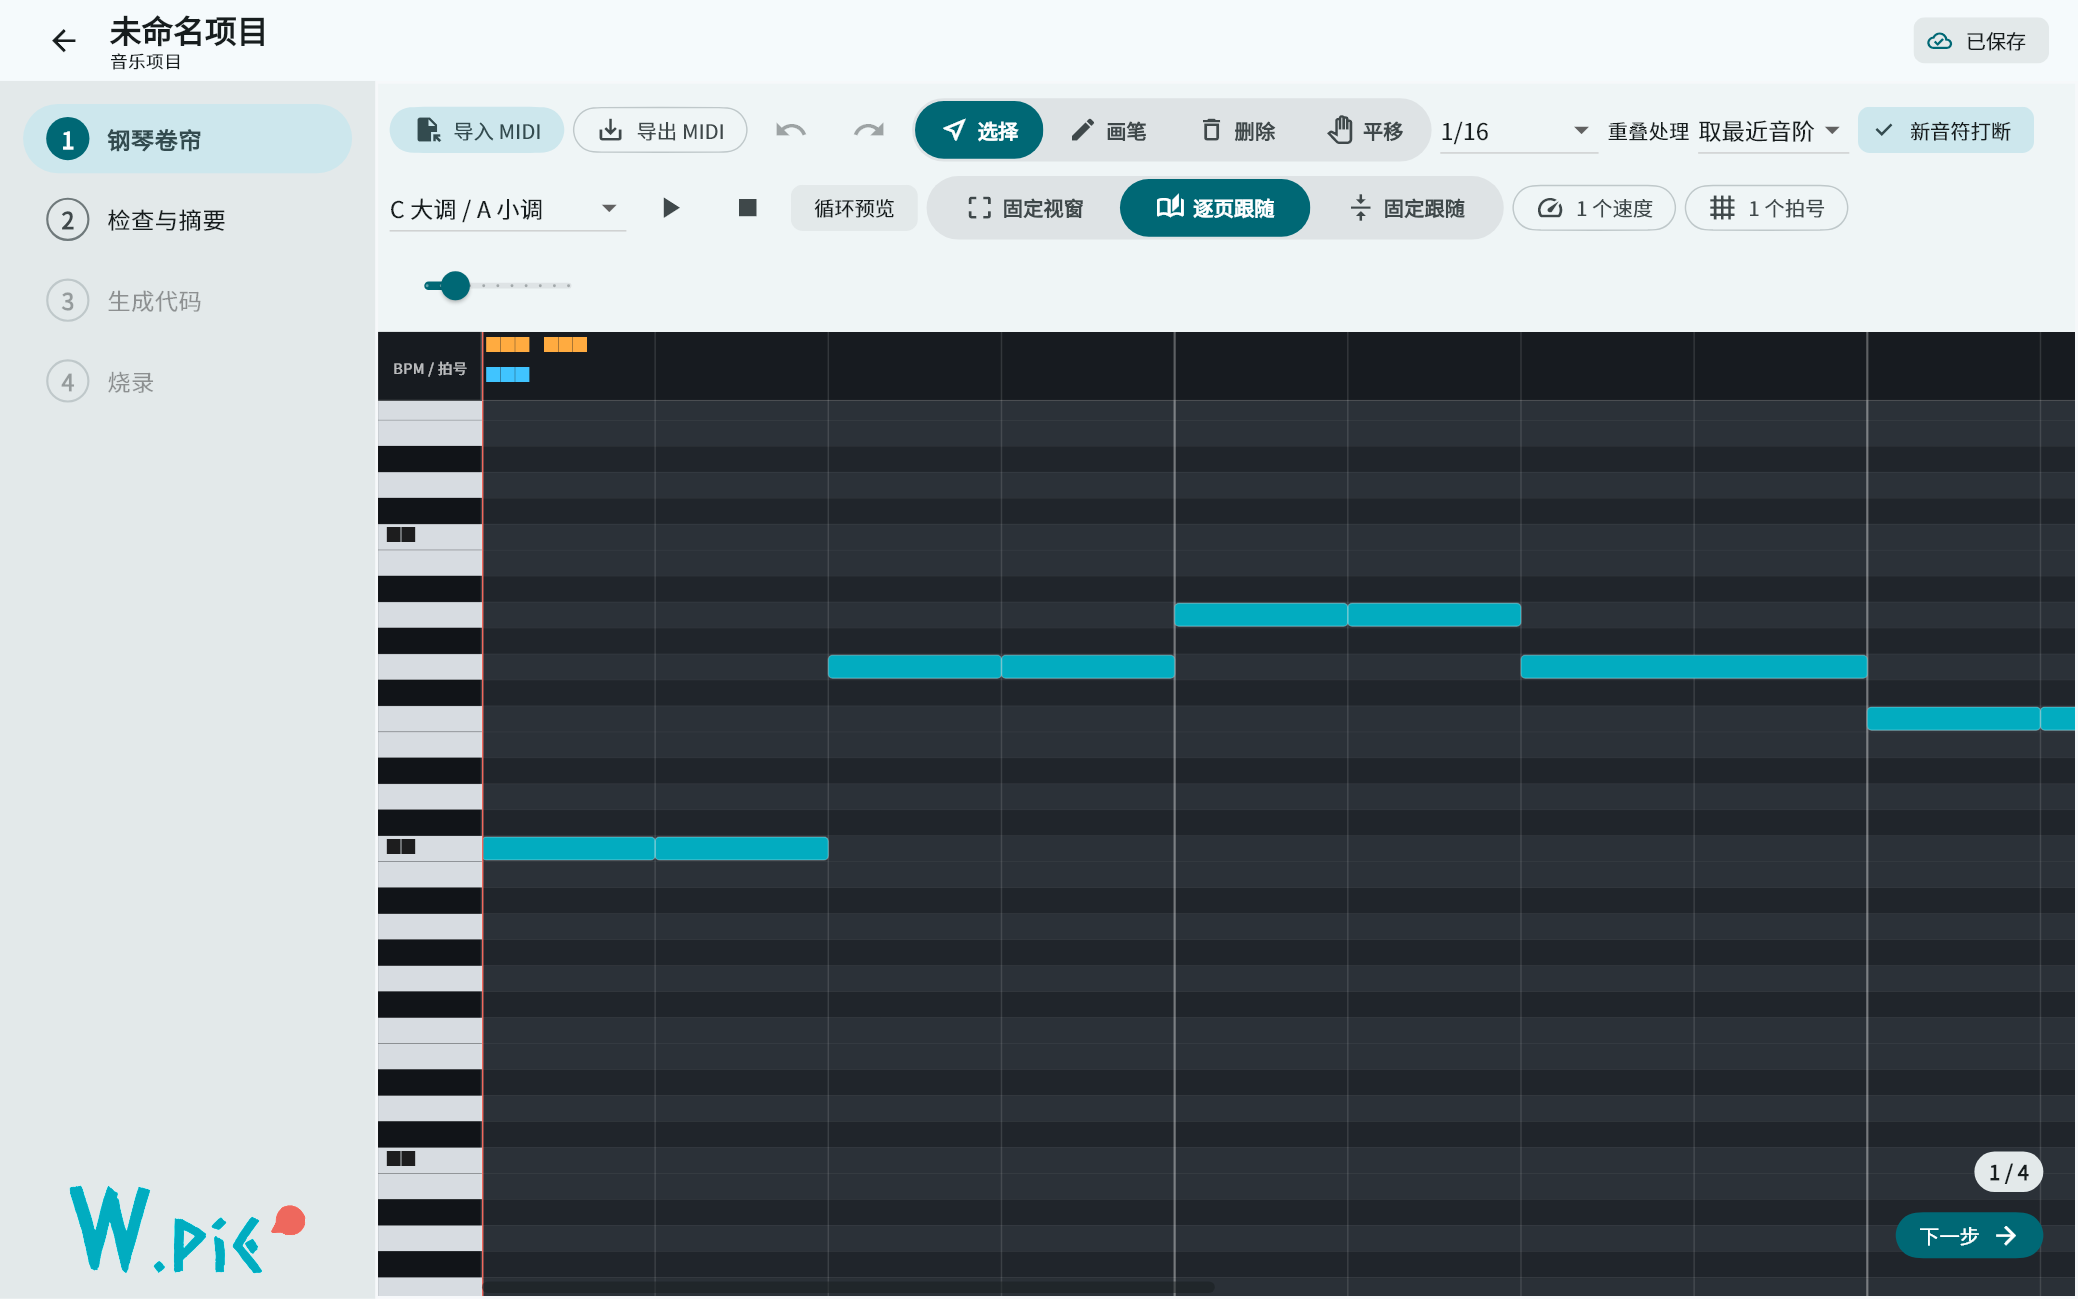
\includegraphics[width=0.98\linewidth]{image/ch07/7-1-music-editor.png}
  \caption{钢琴卷帘编辑器：工具栏、播放控制、速度与拍号事件以及音符区域}
  \label{fig:concise-music}
\end{figure}

工具栏提供四种编辑工具：\textbf{选择}用于点选与框选音符，\textbf{画笔}在网格上新建
音符并拖动改变时值，\textbf{删除}用于移除音符，\textbf{平移}用于整体移动选中的音符。
网格吸附决定新建与拖动对齐的刻度，可选十六分音符、三连音或不吸附。撤销与重做在编辑
过程中始终可用。

播放控制支持从任意位置试听；“循环预览”在编辑区内循环播放；“视窗跟随”让卷帘在播放
时自动跟随当前位置。预览与固件使用同一套发声规则，试听到的效果与主控板一致。

\section{速度与拍号}

工具栏第二行显示乐曲的速度与拍号事件。速度决定演奏的快慢，拍号影响五线谱的分小节
方式与显示。两类事件都从乐曲开头开始，按时间顺序排列；新增或修改后，检查页会核对
顺序是否合法。

初次使用时保持默认值即可，先录入旋律并试听，再根据需要调整速度。改变速度不会改变
音符的相对位置，只改变播放快慢。

\section{重叠处理}

蜂鸣器同一时刻只能发出一个音，而卷帘允许音符重叠。工具栏的“重叠处理”决定重叠时由
哪个音符发声：

\begin{itemize}
  \item \textbf{取最高音}：重叠时音高最高的音符发声；
  \item \textbf{取最低音}：重叠时音高最低的音符发声；
  \item \textbf{取最近音}：选择最接近上一个发声音高的音符，旋律连贯性较好。
\end{itemize}

打开“新音符打断”后，后开始的音符会打断仍在发声的音符，被打断的尾部不再发声。不发声
的音符在卷帘中显示为灰色；数据仍然保留，也参与导出，只是固件不播放。

\section{MIDI 导入与导出}

“导入 MIDI”从标准 MIDI 文件中选择一条旋律轨道，把音符、速度与拍号一并导入。文件里
如果有和弦，导入对话框会要求先选择重叠处理规则，再按规则保留一个声部。没有可用旋律
轨道时，导入会明确报错，不会生成空曲。

“导出 MIDI”把当前卷帘写成标准 MIDI 文件。重叠的完整数据也会写出，灰色音符在音频
软件中仍可编辑。音乐项目不保存原始 MIDI 的力度、乐器与通道信息，导出时值按最终发声
结果计算。

\section{生成与烧录}

音乐项目的“检查与摘要、生成代码、烧录”三步与其他项目一致。检查页会统计音符重叠并
提示采用的规则；曲目过长或音符过多时，会提示缩短乐曲。烧录完成后主控板上电即循环
演奏，内置编译方式下 OLED 屏同步滚动显示五线谱。

蜂鸣器音量有限，适合近距离试听与调试提示，不能替代功率放大后的扬声器。调整曲目后
重新编译烧录即可生效。
